\documentclass[tikz]{standalone}
\usepackage{pgfplots}
\pgfplotsset{compat=newest}
\usepackage{amsmath}
\begin{document}
% defining custom colors
\definecolor{mycolor1}{rgb}{0.49,1,0.63}

\begin{tikzpicture}[node distance = 2cm, auto]
  \node (vd) at (0,0) {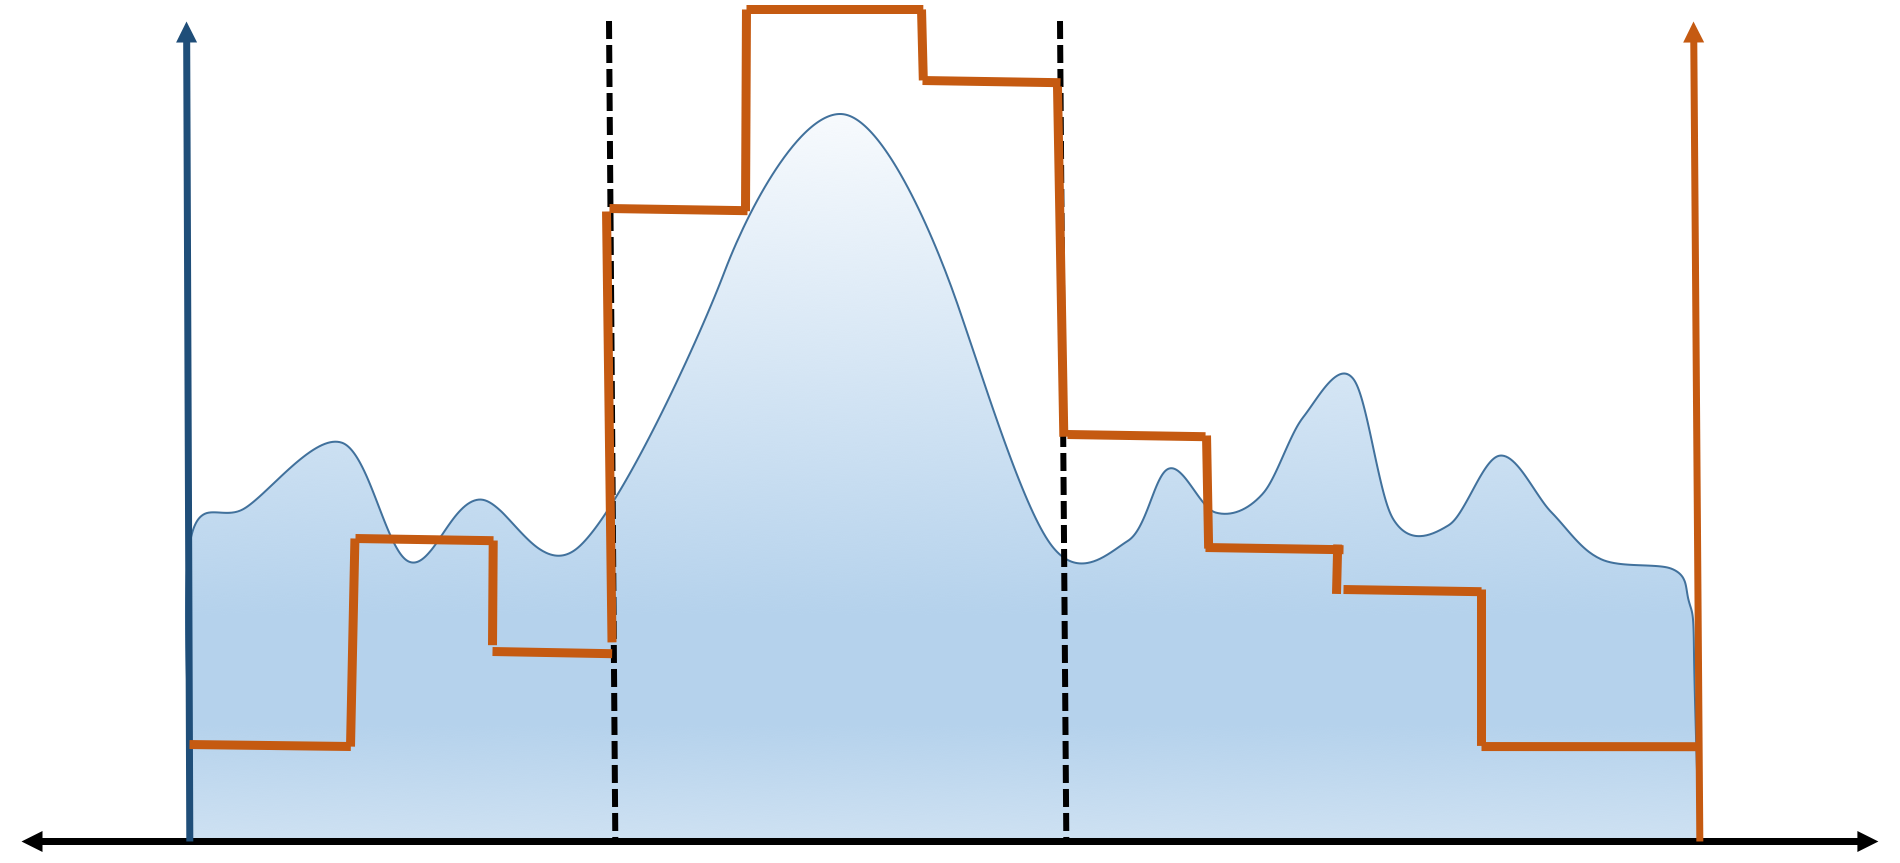
\includegraphics[width=20pc]{scenario2.png}};
  \coordinate [label=left:16:00] (v) at (1.0,-2.1);
  \coordinate [label=left:17:00] (v) at (3.85,-2.1);
  \coordinate [label=right:15:30] (alpha) at (-1.95,-2.1);  
  \coordinate [label=right:15:00] (alpha) at (-3.85,-2.1);
  \coordinate [label=right:Peak disturbance] (alpha) at (-1.8,2.3);
  \coordinate (P) at (-3.6,0);    
  \draw (P) node[rotate=90] (N) {Power Consumption};
  \coordinate (Q) at (3.6,0);    
  \draw (Q) node[rotate=90] (N) {Electricity Price};
  \draw[stealth-stealth, thick] (-1.5, 2) -- (0.5, 2);
  \draw[solid, thick] (0.2, 1.85) -- (1.2, 1.85);
  \draw[solid, thick] (0.2, -1.25) -- (1.2, -1.25);
  \coordinate [label=right:$30\times$, color=red] (v) at (0.7,0.3);
  \draw[stealth-stealth, thick] (0.7, 1.85) -- (0.7, -1.25);
\end{tikzpicture}

\end{document}